% Contesto applicativo

% Stato dell'arte

% Storia e motivi, tutte le volte che il metaverso è stato proposto alla gente e tutte le tecnologie che sono attualmente in uso e anche samsung con il suo vr set del cellulare

\section{Il Metaverso}

    Il concetto di Metaverso deriva dalla fantascienza, infatti il termine fu coniato da Neal Stephenson nel suo libro \textit{Snow Crash} del 1992 dove descriveva uno spazio tridimensionale dove la realtà si univa con un mondo virtuale costantemente attivo.
    %
    Dare una definizione di Metaverso però è molto difficile.
    %
    Spesso le linee di massima di una soluzione futura vengono comprese con largo anticipo ma è impossibile predirre quali caratteristiche conteranno di più, quali modelli si affermeranno o quali dinamiche competitive guideranno la sua formazione.
    %
    Molti tecnologi immaginarono qualche sorta di \textit{Personal Computer} ma la dinamica e il tempismo erano così imprevedibili che nessuno potè immaginare il dominio di Microsoft al posto dell'allora azienda più importante di mainframe, IBM.
    %
    E ancora, nonostante i servizi più usati agli albori di internet furono le mail e la messaggistica istantanea, l'importanza dei social-network non si è capita fino alla seconda metà degli anni 2000.
    
    Allo stesso modo il Metaverso è stato ipotizzato già nei primi anni '80 come una seconda iterazione di internet, ma ancora nessuno può avere la visione completa di cosa sarà. 
    %
    Ad oggi si può dire che il metaverso è il nuovo principale obiettivo delle grandi compagnie di tecnologia mondiali, come Facebook - non a caso rinominata \textit{Meta} - e Epic Games - azienda dietro il motore grafico Unreal Engine e Fortine, il videogioco che ad oggi viene considerato la cosa più vicina al metaverso che sia stata fatta.

    Matthew Ball, CEO di Epyllion e scrittore di \textit{The Metaverse and How it Will Revolutionize Everything}, lo definisce così \cite{Ball2022}: 

    \begin{displayquote}
        \textit{Io definisco il metaverso come un network ampiamente scalabile e interoperabile di mondi virtuali 3D renderizzati in tempo reale che possono essere vissuti, in modo sincrono e persistente, da un numero infinito di user effettivi, ciascuno con un senso di presenza individuale, supportando al contempo continuità di dati quali cronologia, identità, comunicazione, pagamenti, diritti e oggetti.}
    \end{displayquote}

    Secondo Matthew Ball il Metaverso è quindi una combinazione di molte tecnologie diverse che collaborano per costruire un'esperienza continua e persistente.
    %
    È l'unione di mondi virtuali, tecnologie - quali visori per la realtà virtuale, dispositivi indossabili e camere a proiezione 3D - e internet.
    %
    È una nuova era della tecnologia che verrà costruita iteramente e lentamente al di sopra delle tecnologie e dei protocolli esistenti che verranno migliorati o sostituiti in base alle esigenze.
    %
    Un ruolo fondamentale lo avranno le piattaforme virtuali, esse infatti daranno effettivamente vita ai mondi virtuali in cui le persone potranno entrare.
    %
    Alcune hanno scopi puramente di intrattenimento - come Roblox, Legend of Zelda o Minecraft - altri hanno intenti accademici e professionali - come Osso VR o come i simulatori di volo per l'addestramento di piloti.

    La storia del Metaverso è perciò la storia di tutte le tecnologie e le piattaforme online che stanno contribuendo a costruire mondi ed esperienze virtuali.

    \subsection{Storia del metaverso}
    Sebbene il termine fu coniato nel 1992, il concetto di Metaverso affonda le radici ancora prima nella letteratura Cyberpunk.
    %
    Tale letteratura comprende romanzi come \textit{True Names di Vernor Vinge} nel 1981, che descrive quello che può essere considerato il primo esempio di cyber-spazio, e \textit{Neuromancer di William Gibson} nel 1985, che invece ne descrive uno dalle caratteristiche molto simili al Metaverso che intendiamo oggi.

    Il primo dei due libri è particolamente importante perché è stato citato essere la fonte di ispirazione per il primo gioco del Metaverso: Habitat \cite{Habitat1990}.

        \subsubsection{Habitat - la prima implementazione di Cyber-spazio}        

        Nel 1985 le limitate risorse dell'epoca non permettevano stanze virtuali popolose né grafica in 3D, ma Habitat rese possibile per la prima volta a persone da tutto il mondo di incontrarsi in uno spazio virtuale attraverso i propri avatar. 
        %
        Viene definito dai creatori un \textit{ambiente virtuale online multigiocatore} \cite{Habitat1990}, bisognava possedere un Personal Computer che fungeva da frontend e forniva l'interfaccia utente, mentre la comunicazione avveniva su un network a commutazione di pacchetto con un sistema back-end centralizzato.
        %
        L'utente, attraverso il proprio avatar, aveva la possibilità di muoversi nel mondo di Habitat, composto da molte regioni, interagire con oggetti e parlare con altre persone.

        \begin{figure}[h!]
            \centering
            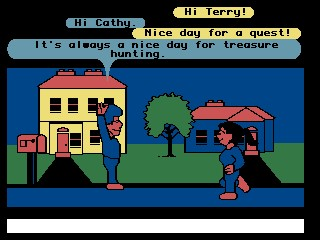
\includegraphics[width=5cm]{figure/lessonshabitat.jpg}
            \caption{Una tipica scena in Habitat.}
        \end{figure}

        Seguirono molti altri con la stessa formula ma Habitat permise per la prima volta di capire a fondo le difficoltà e i requisiti che la creazione di un ambiente virtuale connesso avrebbe avuto. \cite{Habitat1990}
         
        \subsubsection{Second Life}

        Un'altro importante esempio di cyberspazio è Second Life, una piattaforma online lanciata nel 2003.
        %
        Si tratta nuovamente di uno spazio virtuale multigiocatore che grazie alla maggiore disponibilità di risorse che i computer offrivano potè essere sviluppato in 3D.
        %
        In questo mondo le persone possono interagire attraverso i propri avatar con ambienti, oggetti e altre persone, partecipare ad eventi e spostarsi all'interno della mappa di Second Life divisa in \textit{Regioni} (dette \textit{Sim}).
        %
        Ha anche la sua economia interna e un token virtuale a circuito chiuso chiamato \textit{Linden Dollar L\$}. 
        %
        Questa moteva non ha valore monetario ma può essere scambiata con Linden Lab per un corrispettivo in dollari scelto da loro, può essere usata per comprare, vendere, affittare o commerciale beni e servizi con altri giocatori all'interno della piattaforma.
        
        L'importanza di Second Life deriva dal fatto che per la prima volta brand e organizzazioni parteciparono alla realizzazione di oggetti ed eventi nel mondo virtuale portando il gioco a evolversi in qualcosa di più di una pura esperienza d'intrattenimento. 
        %
        Brand come Adidas, Calvin Klein e Lacoste avevano linee di vestiti indossabili dagli avatar dei giocatori \cite{Fascion2nd} mentre alcune università hanno usato Second Life con obiettivi educativi e formativi, incluse l'Università di Harvard e di Oxford \cite{University2ndLife} ma anche alcune italiane come le università di Milano, di Torino, di Salerno e di altre città. \cite{UnitoIn2ndLife, 2ndLifeWikipedia} 
        %
        Ci fu addirittura uno sciopero dei lavoratori IBM organizzato su Second Life nel 2007 che portò migliaia di avatar sulla Sim dell'azienda contemporaneamente. \cite{2ndLifeWikipedia}
        
        \subsubsection{I visori per la realtà virtuale} % qui mettererei i tentativi di samsung

        In \textit{Snow Crash} la tecnologia che permetteva l'accesso al Metaverso erano degli occhiali e degli auricolari, le stesse tecnologie le troviamo anche in altri romanzi come nel più recente \textit{Ready Player One}.
        %
        I visori per la realtà virtuale

    \subsection{Stato dell'arte}

        \subsubsection{Il progetto Oculus}

        \subsubsection{Il piano di Epig Games}

    \subsection{Prospettive future}

        \subsubsection{Lo sviluppo tecnologico}

\section{Il motore grafico Unreal Engine 5}

\section{Il software di modellazione Blender}

    % focus sul progresso tecnologico che resterà nonostante questa sia una bolla finanziaria che scoppierà

    % Metaverso e blockchain hanno ricevuto tantissimi investimenti anche milionari, e sicuramente questo (anche se il mercato delle crypto fallirà) lascerà dei risultati in termini di avanzamento tecnologico

% Pets.com 

% Tedtalk di Talkman premio nobel economia monete e bitcoin

% The line goes up

% Moonekat canale youtube

% Descrizione pura e asettica senza entrare nel dettaglio economico e senza dire che potrà essere una rivoluzione

% Almeno 80 pagine

% .sol per vedere che cos'è uno smart contract

% cosa esce da un'NFT e cosa si vede

